\chapter{Mängder och delmängder}
Mängder och delmängder är ett fundamentallt område inom matematik,
alltså är det väldigt viktigt att kunna detta!
\\\\
En mängd är en samling väldefinierade objekt.
Dessa objekt brukar kallas för \underline{element}.
\\\\
En mängd $A$ bestående av elementen $a_1$, $a_2$, ... , $a_n$ skrivs som $A=[a_1,a_2, ... ,a_3]$.
Om $A$ och $B$ är två olika mängder så betecknar $A\cup B$ alla element som tillhör $A$ eller $B$.
$A\cap B$ alla element som tillhör $A$ \underline{och} $B$.
Konstruktionen $A\cup B$ kallas för \underline{unionen} av $A$ och $B$ och $A\cap B$ kallas för \underline{snittet}.
\\\\
Ett vanligt sätt att visualisera mängder är att genom så kallade \underline{venndiagram}:\\
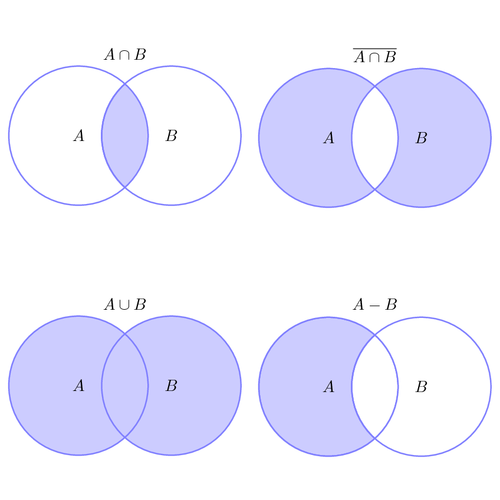
\includegraphics[scale=0.5]{lessons/lesson01/imgs/img01.png}
\clearpage

Ett par saker till
\begin{itemize}
    \item $\emptyset=\{\}$, den tomma mängden
    \item $A^c$ alla element som inte finns i $A$ (kallas \underline{komplementet})
    \item
\end{itemize}

Talmängder är mängder vars element är tal.
Några viktiga talmängder som är grundläggande i matetmatik är:
\begin{itemize}
    \item $\mathbb{N}=\{0,1,2,3,...\}$ de \underline{naturliga talen}
    \item $\mathbb{Z}=\{...,-2-,-1,0,1,2,...\}$ \underline{heltalen}
    \item $\mathbb{Q}=\{\text{Alla talen på formen }\frac{p}{q}\}$, där $p,q\in\mathbb{Z},q\neq 0$
    \item $\mathbb{R}=\{\text{Alla decimaltal}\}$ de \underline{reella talen}
    \item $\mathbb{C}=\{\text{alla tal }a+ib\}$, de \underline{komplexa talen}
\end{itemize}

Inom matematisk analys är mängderna $\mathbb{R}$ och $\mathbb{C}$ speciellt i fokus.

\chapter{Intervall}
Ett \underline{intervall} är en delmängd av $\mathbb{R}$ som innehåller
minst två tal och \underline{alla} tal mellan två av sina element.\\
Mer konkret:\\
\begin{figure}[h!]
    \centering
    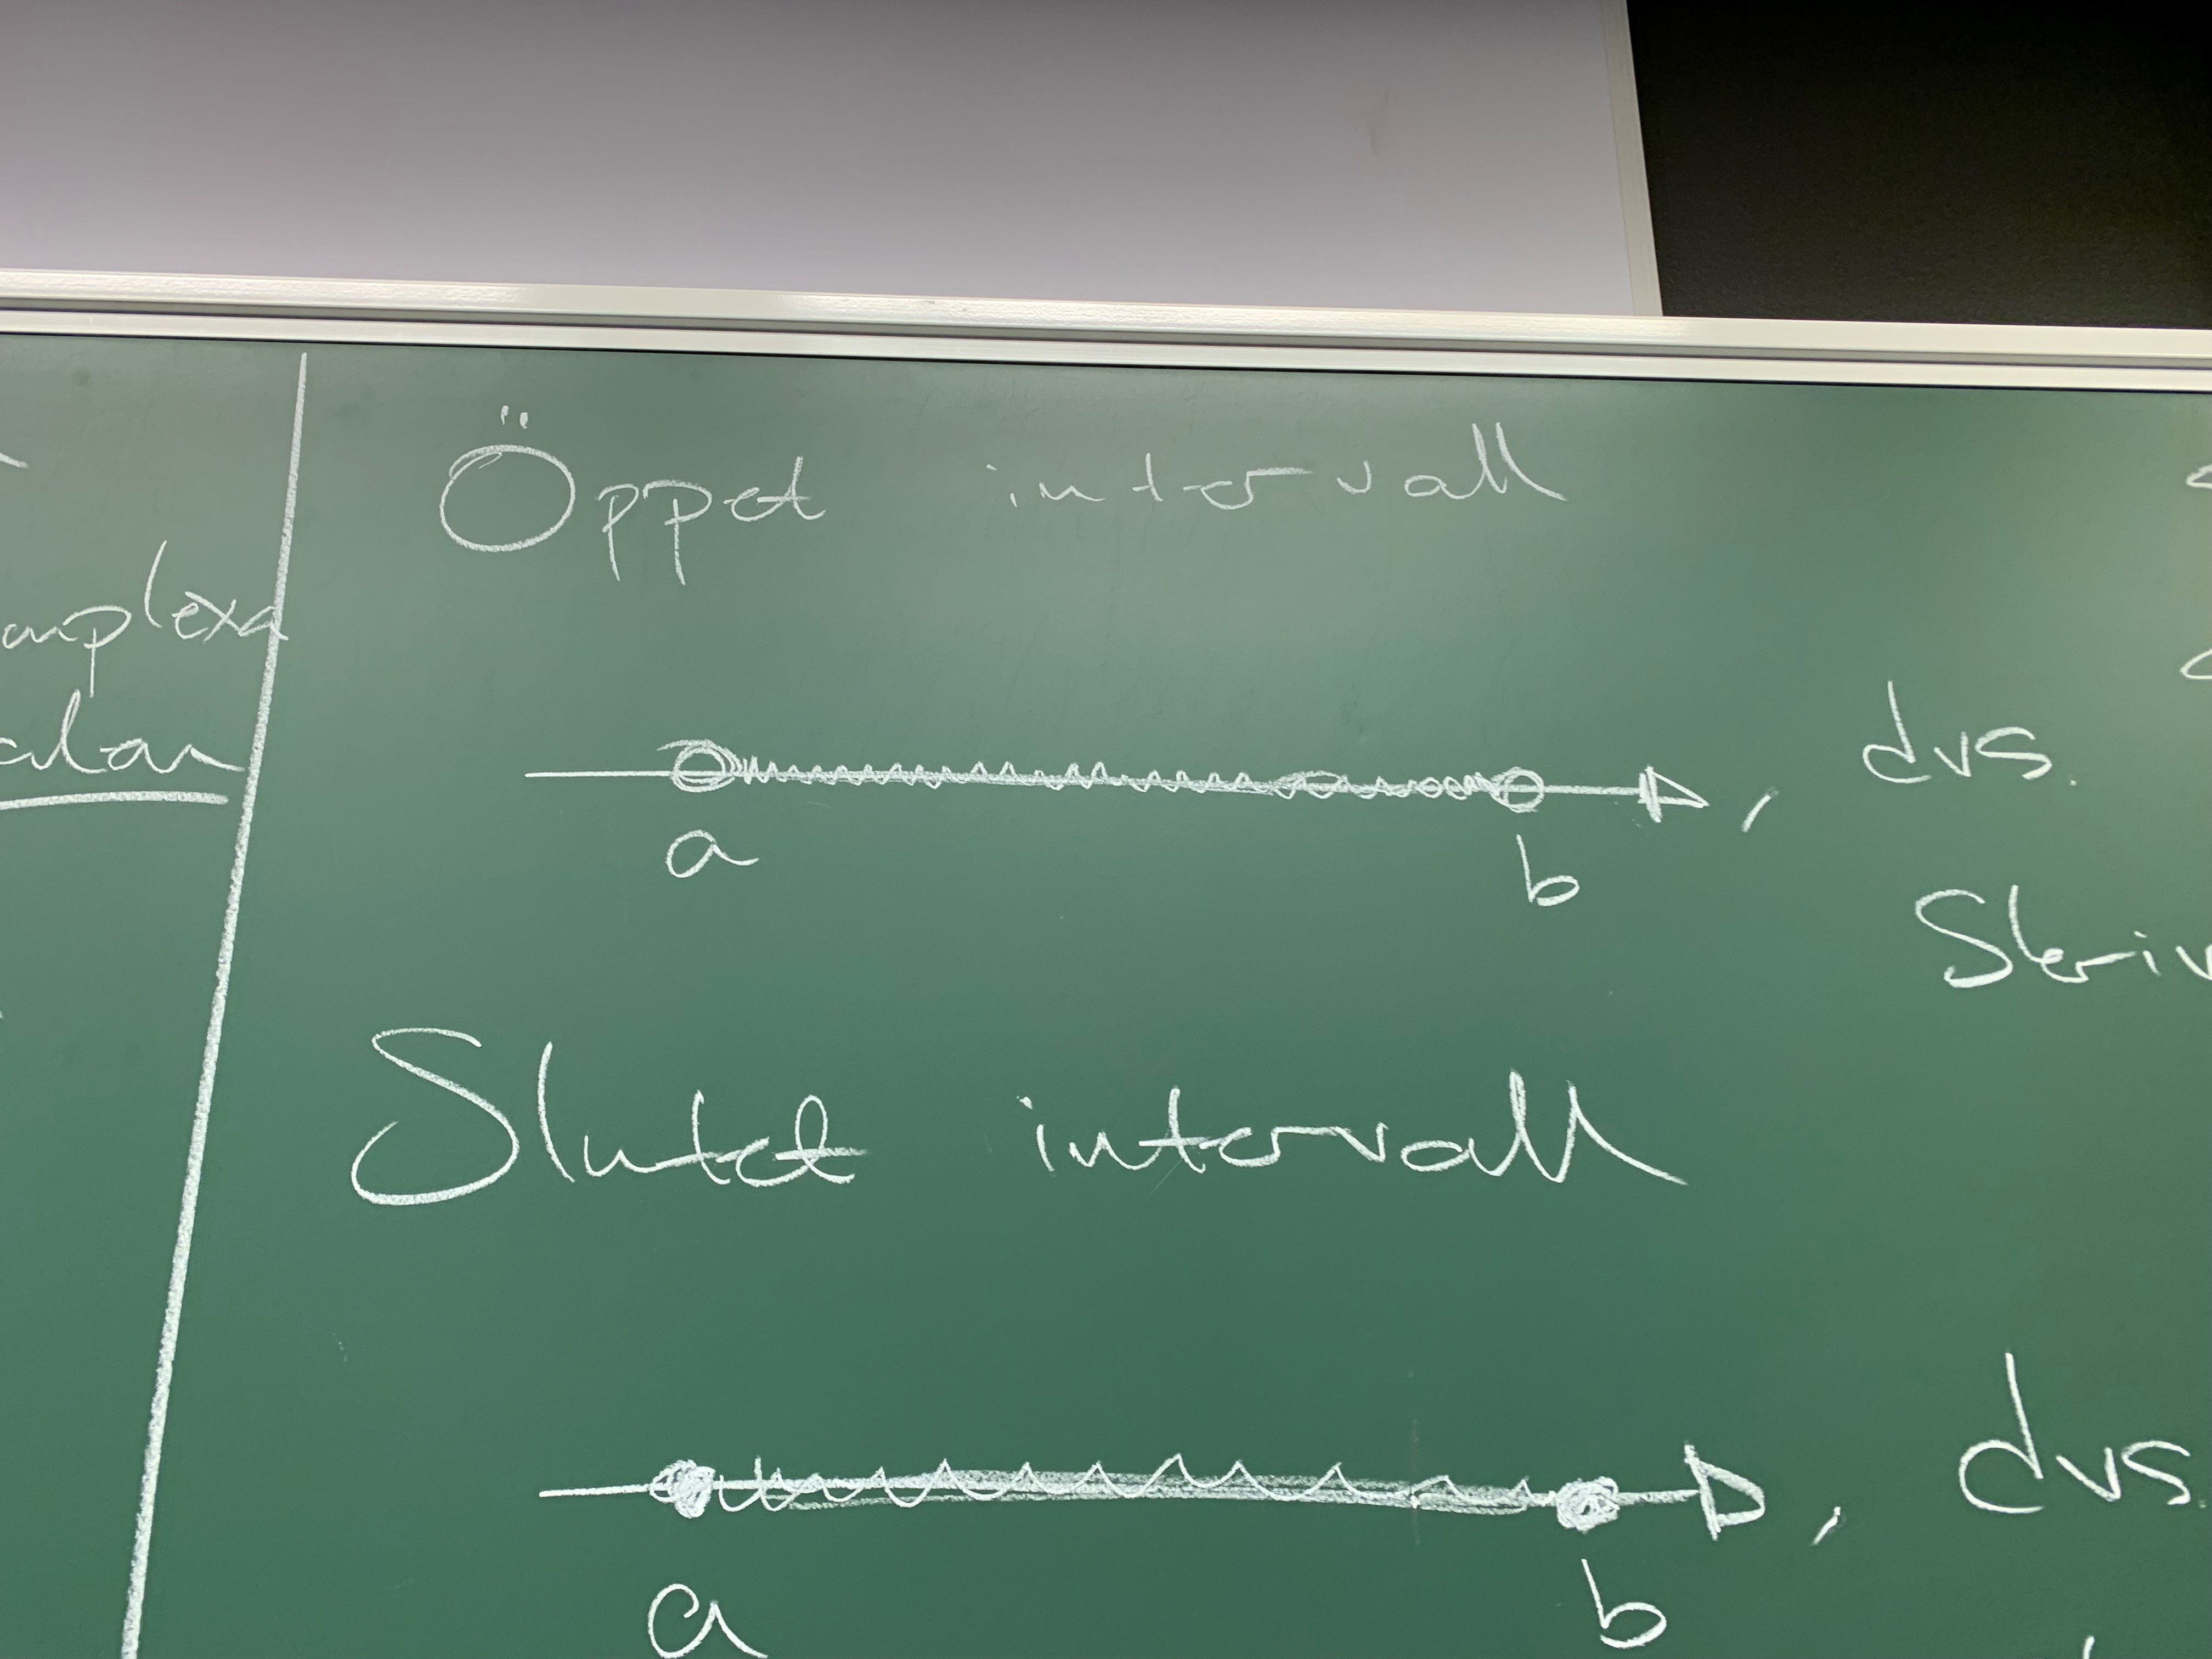
\includegraphics[scale=0.101]{lessons/lesson01/imgs/img02.jpg}
    \caption{$\{x\in\mathbb{R}:a<x<b\}$ skrivs $(a,b)$}
\end{figure}
\begin{figure}[h!]
    \centering
    
\includegraphics[scale=0.08]{lessons/lesson01/imgs/img03.jpg}
    \caption{$\{x\in\mathbb{R}:a\leq x\leq b\}$ skrivs $[a,]$}
\end{figure}
\begin{figure}[h!]
    \centering
    
\includegraphics[scale=0.08]{lessons/lesson01/imgs/img04.jpg}
    \caption{$\{x\in\mathbb{R}:a\leq x\leq b\}$ skrivs $[a,)$}
\end{figure}

\clearpage

\paragraph{Ex}
Lös olikheten $\frac{x}{2}\geq 1+ \frac{4}{x}$ och uttryck svaret som ett intervall eller en union av flera intervall.
\paragraph{Lösning}
Måste försöka skriva om olikheten till faktoriserad form!
\begin{equation*}
    \frac{x}{2}\geq 1+\frac{4}{x}\Leftrightarrow
    \frac{4+x}{x}\Leftrightarrow
    \frac{x}{2}-\frac{4+x}{x}\geq 0\Leftrightarrow
    \frac{x^2-2x-8}{2x}\geq 0
\end{equation*}
Hitta nollställena till $x^2-2x-8$ genom kvadratkomplettering!
\begin{equation*}
    x^2-2x-8=0 \Leftrightarrow
    x^2-2\cdot 1\cdot x+1-1-8=0 \Leftrightarrow
    (x-1)^2-9=0\Leftrightarrow
    x=1\pm \sqrt{9}=1\pm 3\Leftrightarrow
    x=4\text{ eller } x=-2
\end{equation*}
Kan nu skriva om $\frac{x^2-2x-8}{2x}\geq 0$ som $\frac{(x-4)(x+2)}{2x}\geq 0$.
Härifrån kan man använda metoden med teckenstudium:
\begin{equation*}
    \begin{matrix}
                     & \vline &   & -2 &   & 0 &   & 4 &   \\
        \frac{1}{2}x & \vline & - & -  & - & 0 & + & + & + \\
        x-4          & \vline & - & -  & - & - & - & 0 & + \\
        x+2          & \vline & - & 0  & + & + & + & + & + \\
        \text{Tot}   & \vline & - & 0  & + & 0 & - & 0 & +
    \end{matrix}
\end{equation*}
Ser att $\frac{x^2-2x-8}{2x}\geq 0$ uppfylls i intervallen $[-2,0]$ och $[4,\infty)$ och kan skriva lösningen som $[-2,0)\cup[4,\infty)$.
\paragraph{\underline{Absolutbelopp}}
Absolutbelopp av ett tal $x\in\mathbb{R}$ definieras som:
\begin{equation*}
    |x|=
    \left\{\begin{matrix}
        x \text{, om } x\geq 0 \\
        -x \text{, om } x\leq 0
    \end{matrix}
    \right.
\end{equation*}
Följande tolkning gäller:
Givet ett tal $a\in\mathbb{R}$ så gäller för alla $x\in\mathbb{R}$ att $|x-a|=$ avståndet mellan $x$ och $a$.\\
Vidare gäller också, givet ett fixt tal $D\geq 0$, att
$|x-a|\begin{matrix}< \\=\\>\end{matrix}D\Leftrightarrow$
mängden av alla $x\in\mathbb{R}$ vars avst. till $a$ är $\begin{matrix}<\\=\\>\end{matrix}D$,
dvs $|x-a|\begin{matrix}< \\=\\>\end{matrix}D\Leftrightarrow\begin{matrix}
        a-D<x<a+D \\
        x=a-D     \\
        x<a-D,x>a+D
    \end{matrix}$

\clearpage

\paragraph{Ex} (P1.41)\\
Lös olikheten $|x+1| >|x-3|$ genom att tolka avs som ett avst. på talaxeln.
\paragraph{Lösning}~\\
$|x+1| = |x-(-1)|=$ "avst mellan $x$ och $(-1)$"\\
$|x-3|=$ "avst. mellan $x$ och $3$"\\
Så "avst. mellan $x$ och $(-1)$" $ > $ "avst. mellan $x$ och $3$"\\
Till höger om $1$ så kommer $x$ \underline{alltid} att vara längre från $(-1)$ än $3$.
\begin{figure}[h!]
    \centering
    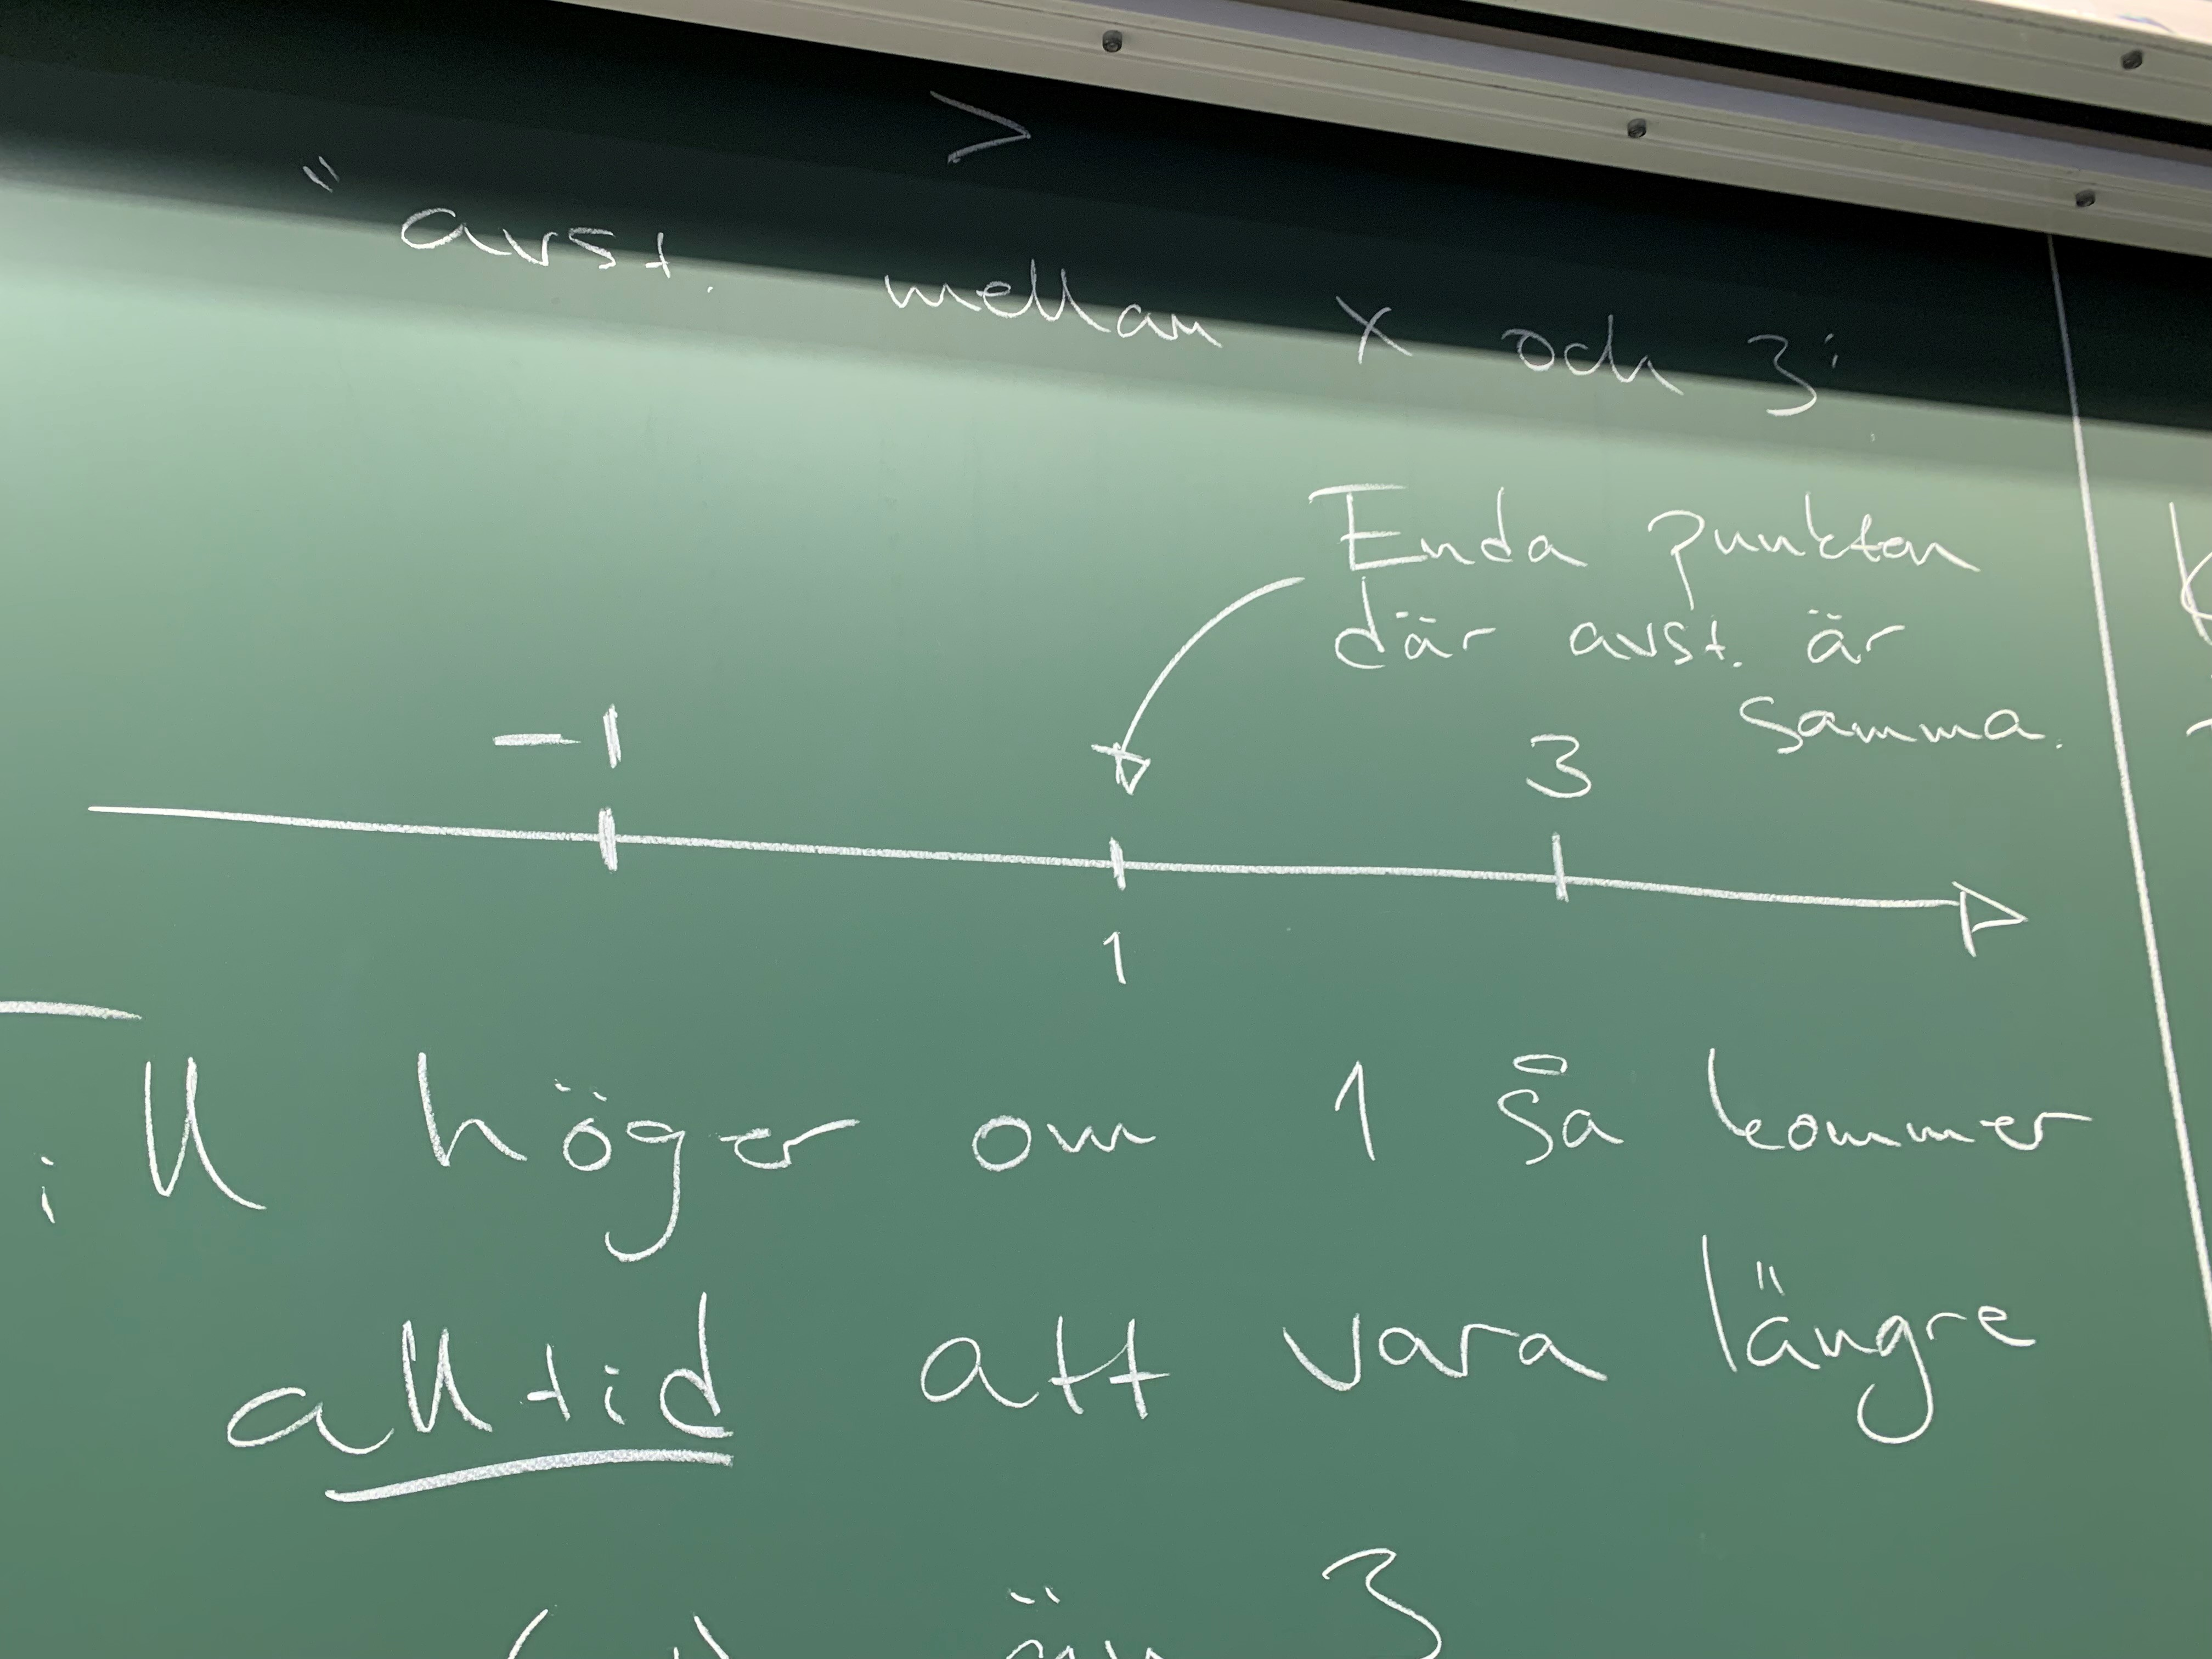
\includegraphics[scale=0.08]{lessons/lesson01/imgs/img05.jpg}
    %\caption{}
\end{figure}

\chapter{Komplexa tal}
Ett komplext tal $z\in\mathbb{C}$ kan alltid skrivas på formen $z=a+i\cdot b$ där\\
\begin{itemize}
    \item $a$ kallas för \underline{realdelen} av $z$ $Re(z)$
    \item $b$ kallas för \underline{imaginärdelen }av $z$ $Im(z)$
\end{itemize}

Den imaginära enheten $i$ löser definitionsmässigt ekv. $x^2+1=0$, dvs $i=\sqrt{-1}$.
Rent visuellt kan man betrakta ett komplext tal $a + ib$ som en punkt i det komplexa talplanet.\\
Det gäller att $r^2= |a+ib|^2= \vdots =a^2+b^2$.
Givet $r$ och argumentet $\theta$ kan \underline{alla} kompexa tal skrivas $z=r(cos(\theta)+i\cdot sin(\theta))$
%infoga bild 6
\begin{figure}[h!]
    \centering
    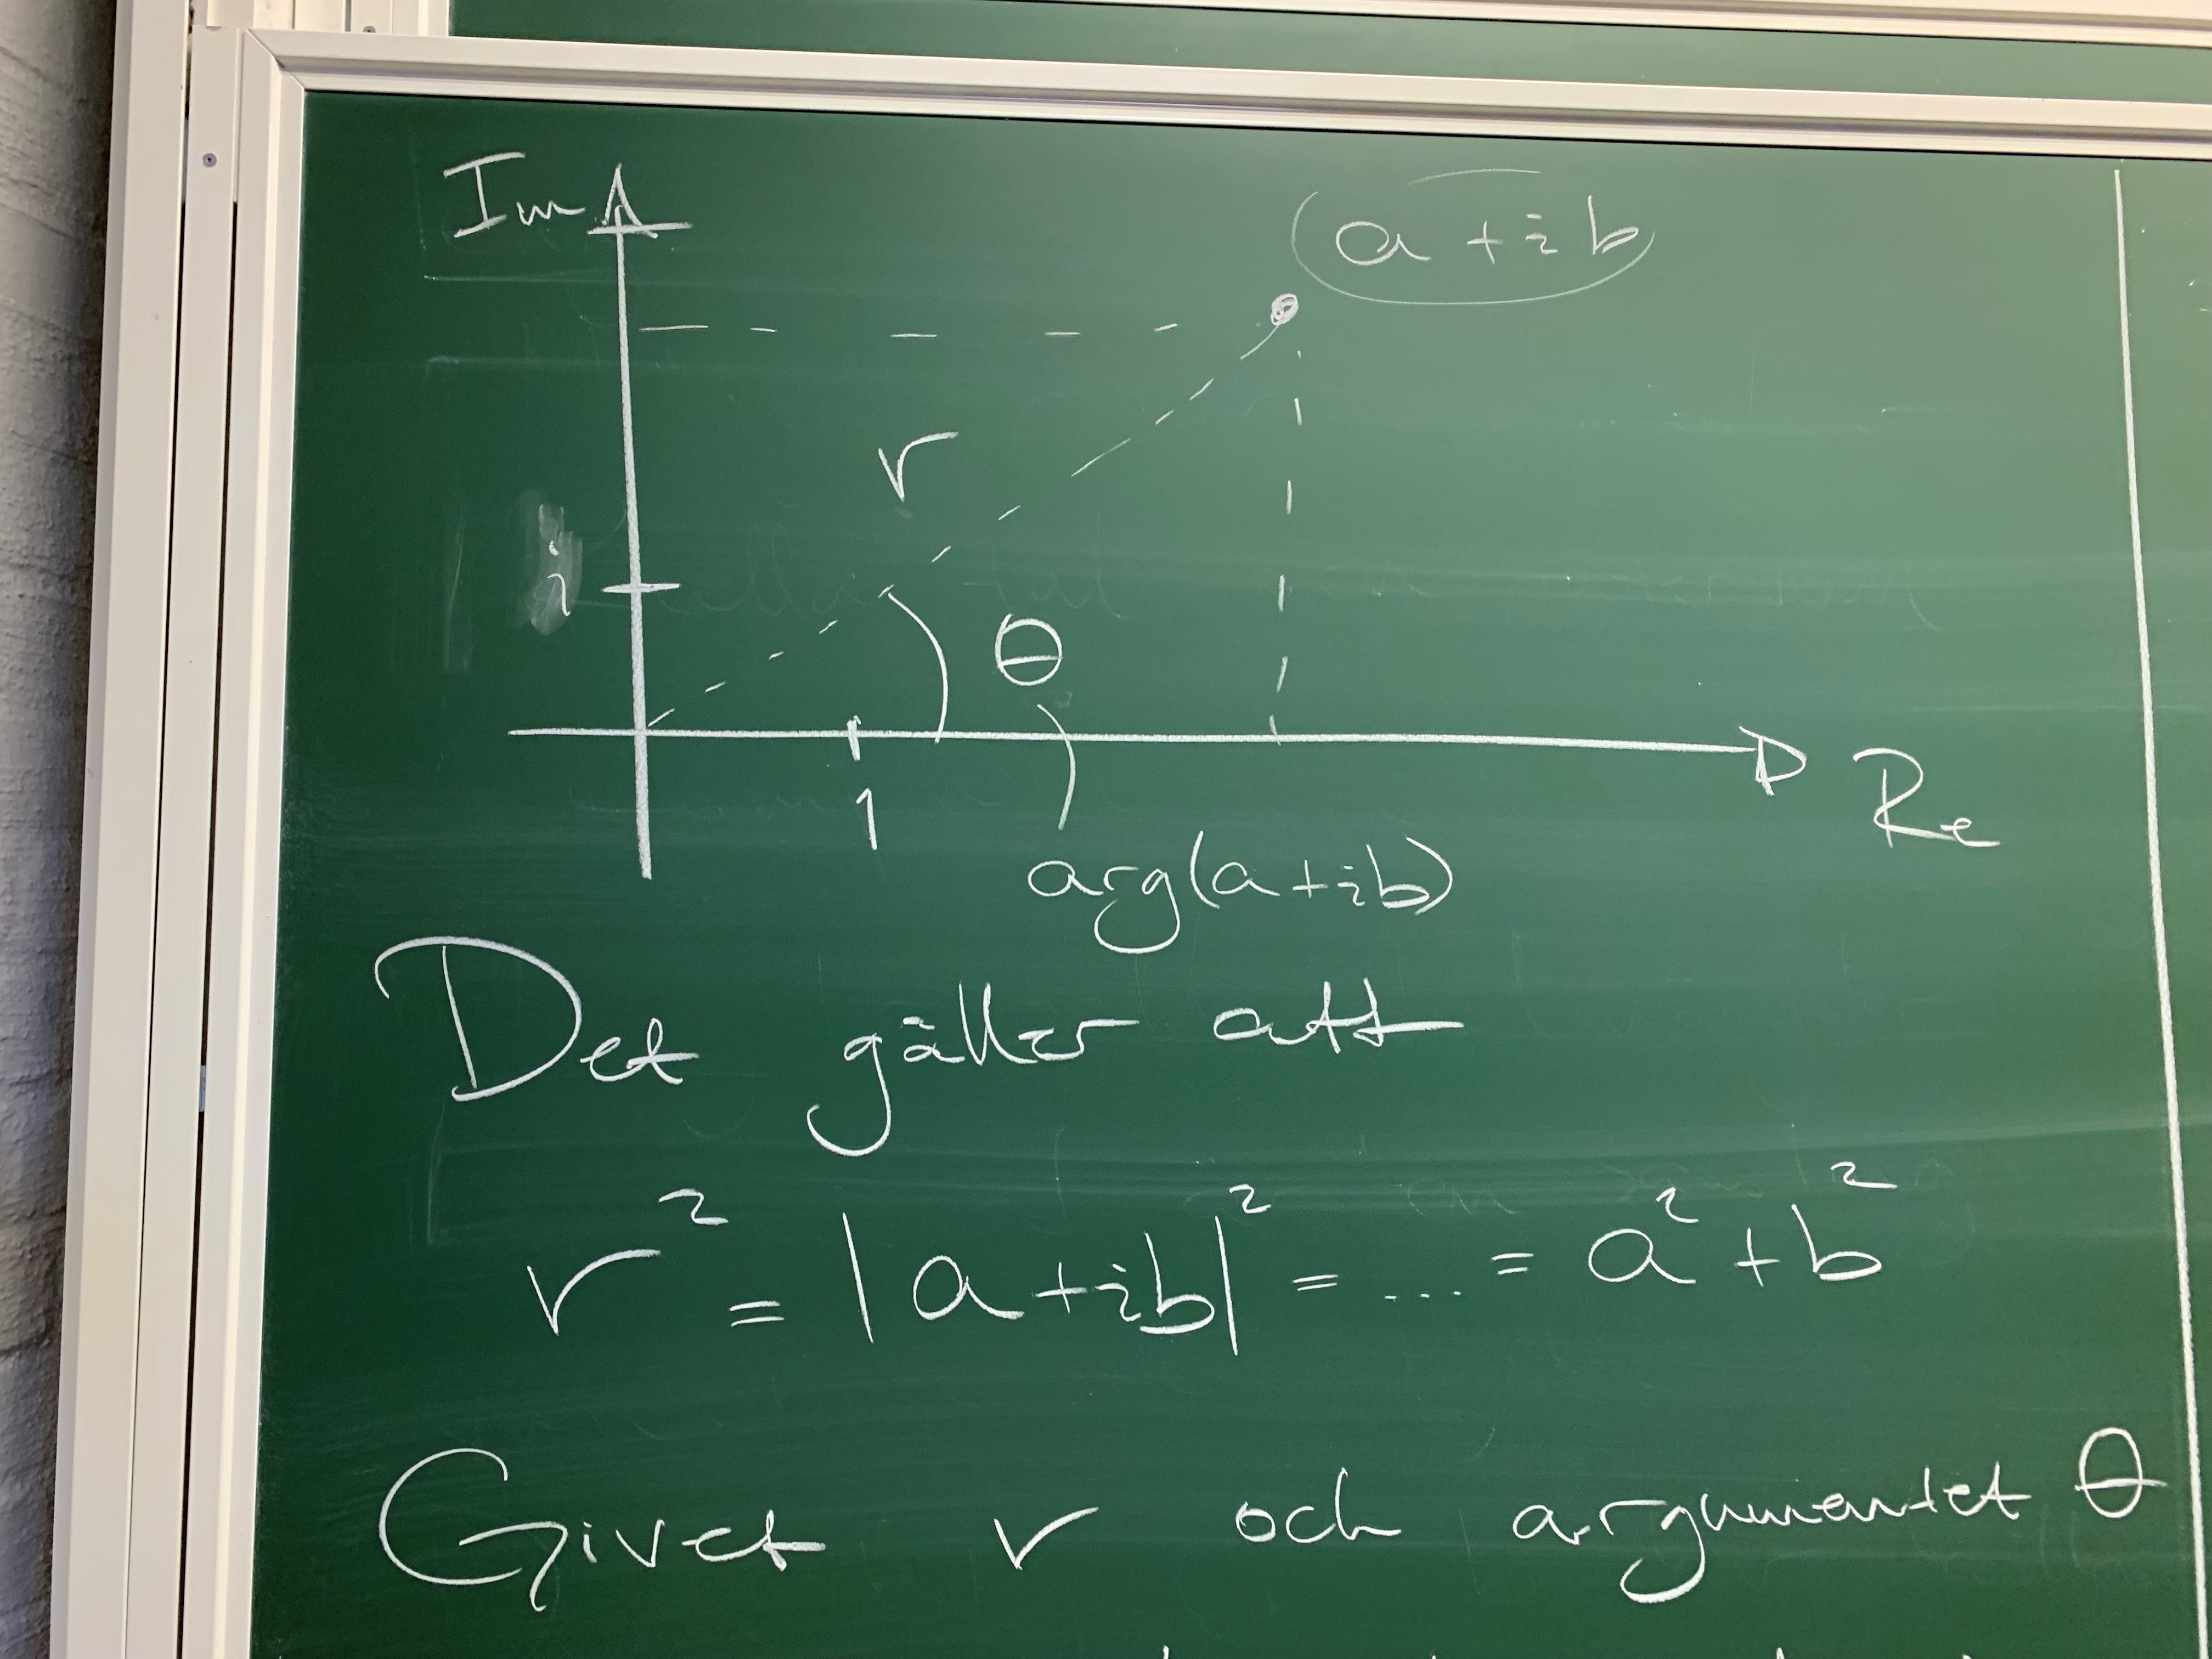
\includegraphics[scale=0.08]{lessons/lesson01/imgs/img06.jpg}
    %\caption{}
\end{figure}